\frontmatter
%███████████████████████████████████████████████████████████████████
%███████████████████████████████████████████████████████████████████
%███████████████████████████████████████████████████████████████████
\chapter{Intro}

Classical physics accurately predicts the movement of objects in our everyday world. However, there are effects that it does not account for, and as objects approach the speed of light, these effects that are negligible at low speeds become increasingly significant. This leads to two observers moving at high speeds relative to each other becoming unable to agree on the lengths of objects and the times in which events occur. Crucially though, one thing remains constant: the speed of light relative to each observer is the same, regardless of their movement. We must redefine our understanding of time and space to find out how this can be. This is where special relativity comes into play.

Special relativity is vital in particle, nuclear, and astrophysics, used for calculating nuclear reaction output power and measuring galaxy speeds. It is also needed for precision timekeeping on fast-moving GPS satellites to calculate positions accurately.


Despite its importance, special relativity continues to confuse even those well-versed in physics and mathematics. It can be as confusing to visualize and understand as quantum mechanics is. The theory requires letting go of some deeply held intuitions about the absolute nature of space and time that differ from our usual everyday experience of the physical world.

% EDIT: Next paragraph is a bit stale
This handbook is meant to offer an intuitive, visual, and comprehensive overview. The aim is to maintain simplicity and avoid unnecessary abstraction in explanations. For example, time in diagrams is shown either using animations or multiple diagrams given one after another in a timeline. This approach avoids the use of unnecessary space-time diagrams, which represent time on one of the axes and make special relativity more abstract and confusing to visualize.

% Next bit feels like a bit of a lie as i have coordinate axis in overview and some math terms % can change the inertial reference frame section though instead
The first chapter is readable even for those without a math or physics background. It provides a non-mathematical, visual overview of the concepts. This chapter builds an intuitive understanding of the core ideas step-by-step, providing a solid foundation for developing the essential mathematical framework in later sections. The mathematical portion will begin with deriving how space and time coordinates function in special relativity. This will be followed by velocity addition, the Doppler effect, and the energy-momentum relationship. In addition to these topics, we will also explore some interesting subjects not typically covered in standard resources. These include how a source’s emitted light is concentrated in the direction of its movement, aberration, and how a delay in light signals leads to retarded source positions and fields. These topics will probably not mean much to you yet, but they will give interesting insights.

%the Liénard-Wiechert-Potentials, maybe quaternions in SR if you are lucky, and so on.
% Your momma did not raise you right, so it is my turn to whip you into shape. By the end of this book, you will also be able to understand yourself a little more (because there will be a subsection on retarded jerks). You already have something in common with this topic of relativity because you are special!... The only thing that can undo Lorentz length contraction is your momma
% This book is not an inertial frame of reference unless in free fall (but gravity, which is for a different day). Damage caused to this book by allowing it to enter a short-lived inertial frame of reference before making an abrupt exit is not covered by our returns policy (do not throw the book at the ground!). \\

\newpage

\begin{figure*}
    \centering
    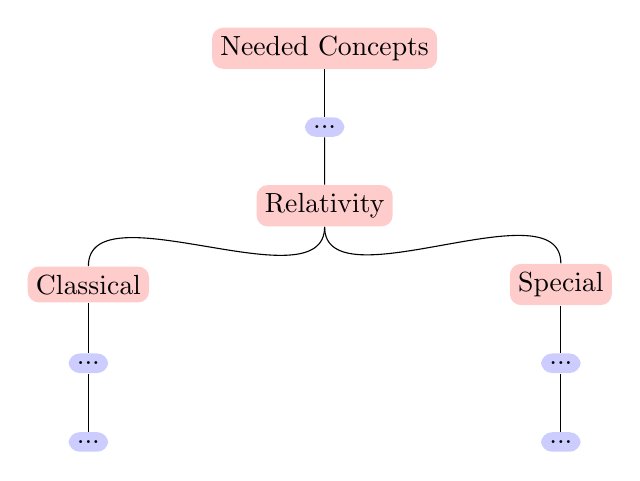
\begin{tikzpicture}[level distance=10mm, sibling distance=20mm,
        edge from parent path=
      {(\tikzparentnode.south) .. controls +(0,-1) and +(0,1)
                                 .. (\tikzchildnode.north)},
        mynode/.style={fill=blue!20,rectangle,rounded corners,inner sep=3pt,align=center},
        rednode/.style={fill=red!20,rectangle,rounded corners,inner sep=3pt,align=center}
        ]
        %mynode/.style={draw,circle,inner sep=2pt,align=center}
        %mynode/.style={draw,rectangle,rounded corners,inner sep=2pt,align=center}
      ]
        \node[rednode] {Needed Concepts}
          child {node[mynode] {...}
            child {node[rednode] {Relativity}
              child [sibling distance=60mm] {node[rednode] {Classical}
                child {node[mynode] {...}
                  child {node[mynode] {...}}
                }
              }
              child [sibling distance=60mm] {node[rednode] {Special}
                child {node[mynode] {...}
                  child {node[mynode] {...}}
                }
              }
            }
          };
      \end{tikzpicture}
\end{figure*}

%\vspace{1cm} \newline
Now, let us begin!

\newpage